\section{Problem Statement}

A general purpose framework should be configurable for multiple use cases in its designated domain. CouchEdit as a general purpose graphical modeling framework thus should be configurable for multiple modeling syntaxes. Technically this is possible, as long as one has access to the source code. But this would mean, every time CouchEdit has to support a new modeling syntax, manual changes in the source code have to be made and the project has to be compiled from sources. The implementation of a configuration parser, that can interpret modelling syntax definitions at runtime would thus increase flexibility. Furthermore a well designed metamodel could reduce the amount of knowledge that is needed about the CouchEdit framework.

As a relaxed conformance editing framework, CouchEdit poses special architectural requirements. It has to allow for temporary inconsistencies between concrete syntax (what the user draws) and abstract syntax (what the underlying Model actually looks like). As the concrete syntax does not always have to map to a syntactic correct abstract model, this allows for more freedom in the modeling process (e.g. dangling transitions).

CouchEdit achieves this by building upon the architecture concept of clear separation between concrete and abstract syntax, proposed by Y. Van Tendeloo et al. \cite{van_tendeloo_concrete_2017}. Internally, CouchEdit builds a hypergraph, that maps the given concrete syntax to all possible abstract syntaxes (interpretation of a concrete syntax can be ambiguous and thus multiple abstract syntaxes can be possible). To build this Hypergraph, a set of Processors is employed, which are connected in a reactive publish and subscribe pattern. All Processors (and the user interface) are subscribed to a bus (fig. \ref{fig:processors}). If a change (diff) is published to the bus (e.g. the user adds a node to the concrete syntax), all processors that are subscribed to this type of diff are notified and calculate new resulting diffs, these new diffs are then also published to the bus and all processors interested in them are invoked as well.

\begin{figure}
  \centering
  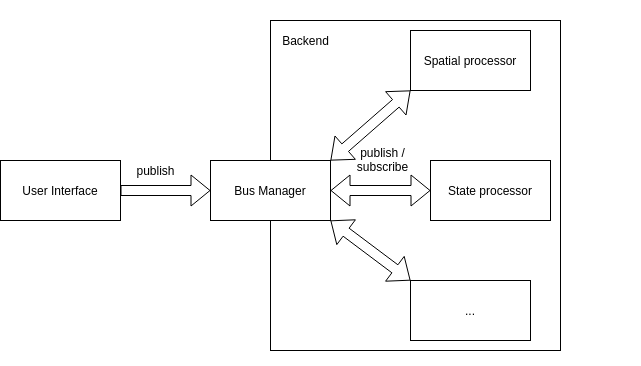
\includegraphics[width=.6\linewidth]{images/couchedit-processors}
  \caption{Publish Subscribe architecture of CouchEdit}
  \label{fig:processors}
\end{figure}

Some of these processors are needed for every type of syntax model, for example the spatial processor, that processes how nodes in the concrete syntax are positioned to each other (above, besides, etc.). Other processors are specific to the given modeling syntax, for example a state chart syntax would require a state processor, that processes if a given graphical object represents a state (usually true if the given node is a rectangle with rounded edges).

A modeling syntax parser for CouchEdit would have to generate these syntax specific processors, while considering multiple design constraints that result from this architecture. Thus a metamodel is needed that can define the desired abstract modeling syntax and specify how a concrete graphical syntax can be mapped to this abstract syntax. While there is ongoing research in the area of relaxed conformance editing and how to link concrete and abstract syntax, it does not immediately become clear what such a metamodel would look like.
